%
% HSR LaTex Template
% Copyright 2012, Florian Bentele
%
% Complete LaTex template for thesis at HSR, customized
% for Prof. Dr. Peter Heinzmann
%
%
% This document is free software: you can redistribute
% it and/or modify it under the terms of the GNU
% General Public License as published by the Free
% Software Foundation, either version 3 of the License,
% or (at your option) any later version.
%
% This document is distributed in the hope that it will
% be useful, but WITHOUT ANY WARRANTY; without even the
% implied warranty of MERCHANTABILITY or FITNESS FOR A
% PARTICULAR PURPOSE. See the GNU General Public
% License for more details.
%
% You should have received a copy of the GNU General
% Public License along with this document. If not, see
% <http://www.gnu.org/licenses/>.
%
\documentclass[11pt,twoside]{hsrthesis}

\makeindex
%add new glossaryentries here...
\newglossaryentry{dropwizard}{name=Dropwizard,description={Das Framework Dropwizard.io erlaubt eine einfache Implementation von RESTFull Web Services. Dropwizard verbindet verschiedene Technologien wie JAX-RS mit Jersey, Jackson, Netty Server usw., um ein Paket für den Entwickler zu erstellen, welches einfach implementiert und deployed werden kann.\\ (\href{http://www.dropwizard.io/}{http://www.dropwizard.io/})},first={Dropwizard}}

\newglossaryentry{playframework}{name=Play Framework,description={Das Play Framework ist ein Opensource Projekt, mit dem Ziel, ein einfaches und leichtgewichtiges MVC Framework zu bieten. Play wird mit einem Netty Server ausgeliefert und muss daher nicht installiert werden (\href{https://www.playframework.com}{https://www.playframework.com})},first={Play Framework}}

\newglossaryentry{postgresql}{name=PostgresSQL,description={PostgreSQL ist eine relationale Opensource Datenbank (\href{http://www.postgresql.org/}{http://www.postgresql.org/}) },first={PostgreSQL}}

% do this here, so you can \gls{...} to it
\makeglossaries

\begin{document}

\newcommand{\thesistitle}{Verkehrsmodell-Fallstudien-Editor}
\newcommand{\thesisauthora}{Fabian Keller}
\newcommand{\thesisauthorb}{Dominik Heeb}
\newcommand{\thesisauthorc}{}
\newcommand{\professor}{Prof. Dr. Luc Bläser}
\newcommand{\thesistype}{Bachelorarbeit}
\newcommand{\departement}{Abteilung Informatik}
\newcommand{\school}{Hochschule für Technik Rapperswil}
\newcommand{\term}{Frühlingssemester 2016}
\newcommand{\thedate}{17. Juni 2016}
\newcommand{\timeperiode}{22.02.2016 - 17.06.2016}
\newcommand{\partner}{Dr. Marcel Rieser, Senozon AG}
\newcommand{\workload}{360 Stunden, 12 ECTS pro Student}

\setlength{\oddsidemargin}{20mm}
\maketitle
\setlength{\oddsidemargin}{20mm}


\tableofcontents


% The main content
%%%%%%%%%%%%%%%%%%
\chapter{Abstract}
\begin{flushleft}
TODO
\end{flushleft}



\chapter{Einführung}

\section{Senozon AG}
Diese Bachelorarbeit wird in Zusammenarbeit mit dem Unternehmen Senozon AG durchgeführt. Die Senozon AG ist ein international tätiges Technologieunternehmen auf dem Gebiet der Standortplanung und -bewertung, Verkehr- und Infrastrukturplanung sowie Mobilitätsforschung. Dafür unterhält die Senozon AG verschiedene Verkehrsmodelle, die im Wesentlichen aus einem Strassennetz, ÖV-Fahrplan und Personendaten bestehen, wobei letztere die Reiseaktivität der Personen beschreiben.
\section{MATSim Framework}
Die Senozon AG verwendet für die Simulation der verschiedenen Verkehrsmodelle das Open Source Framework MATSim.\\
MATSim ist ein modular aufgebautes Tool zur agentenbasierten Mobilitätssimulation, welches besonders für grosse Szenarien mit Millionen von Agenten (Personen) geeignet ist. Zudem kann sowohl privater als auch öffentlicher Verkehr (Bus, Zug, Tram usw.) simuliert werden.\\
Die Senozon AG stellt zusammen mit der ETH Zürich, der TU Berlin und vielen anderen Universitäten die Weiterentwicklung und Qualitätssicherung von MATSim sicher.
\chapter{Problemstellung}

\section{Senozon AG}
Diese Bachelorarbeit wird in Zusammenarbeit mit dem Unternehmen Senozon AG durchgeführt.\\
Senozon ist ein international tätiges Technologieunternehmen auf dem Gebiet der Standortplanung und -bewertung, Verkehr- und Infrastrukturplanung sowie Mobilitätsforschung. Dafür unterhält Senozon verschiedene Verkehrsmodelle, die im Wesentlichen aus einem Strassennetz, ÖV-Fahrplan und Personendaten bestehen, wobei letztere die Reiseaktivität der Personen beschreiben.
\section{MATSim Framework}
Die Senozon AG verwendet für die Simulation der verschiedenen Verkehrsmodelle das Open Source Framework MATSim.\\
MATSim ist ein modular aufgebautes Tool zur agentenbasierten Mobilitätssimulation, welches besonders für grosse Szenarien mit Millionen von Agenten (Personen) geeignet ist. Zudem kann sowohl privater als auch öffentlicher Verkehr (Bus, Zug, Tram usw.) simuliert werden. MATSim arbeitet leider noch Dateibasiert. D.h. alle Informationen für die Simulationen werden...
Die Senozon AG stellt zusammen mit der ETH Zürich, der TU Berlin und vielen anderen Universitäten die Weiterentwicklung und Qualitätssicherung von MATSim sicher.\\
\section{Detaillierte Problemstellung}
\subsection{Allgemein}
TODO
\subsection{Problem Datenfiles}
TODO
\subsection{Änderungsmanagement}
TODO




\chapter{Anforderungen \& Analyse} \label{ch:anforderungen_section}
\section{Anforderungen}
\subsection{Funktionale Anforderungen}
\begin{flushleft}
TODO
\end{flushleft}
\subsection{Nicht funktionale Anforderungen}
\begin{flushleft}
TODO
\end{flushleft}
\section{Analyse}
\subsection{Risiken}
\begin{flushleft}
TODO
\end{flushleft}
\chapter{Konzepte \& Architektur}
\label{ch:konzepte_architektur}
\section{Konzepte}
Für die Bewältigung der Anforderungen an die Softwarelösung wurden Konzepte entwickelt, welche Einfluss auf die einzelnen Komponenten und die Architektur haben. Die Softwarelösung soll wie unter Kapitel \ref{ch:anforderungen_section} \nameref{ch:anforderungen_section} beschrieben,  die Möglichkeit bieten, Simulationsdaten auf einer Karte darzustellen, sowie auch deren Bearbeitung ermöglichen. Wichtig ist dabei, dass die Bearbeitung keinen Einfluss auf die Stammdaten hat. Die dafür benötigten Konzepte, werden in diesem Kapitel beschrieben.
\subsection{Daten QuadTiles}
\label{ch:datentiles}
Der Umgang mit der grossen Datenmenge (ca. 4 Millionen Datensätze für die Schweiz) ist eine grosse Herausforderung dieser Arbeit. Um diese grosse Datenmenge zu bewältigen, wurde ein bewährtes Verfahren für die Kartendarstellung verwendet. Dies ist der QuadTile Algorithmus von OpenStreetMap \citep{OSMQuadTiles}. Dabei werden die Daten nicht als Gesamtes geliefert, sondern über Teilbereiche, sogenannte Tiles, angefragt. Ein Tile ist ein Quadrat, welches ein vordefinierten Bereich der Welt abdeckt. Dies ermöglicht es einzelne Bereiche (Tiles), die zur Zeit angezeigt werden, zu laden und nicht immer den kompletten Datenstamm. Ein weiteres Konzept, in Verbindung mit dem QuadTile Algorithmus, wird unter Kapitel \ref{sec:concept_preprocessing} \nameref{sec:concept_preprocessing} beschrieben. Dabei werden die Daten für jede Zoomstufe bewertet und lediglich bei Relevanz mitgeliefert. Durch diese beiden Konzepte kann die Datenmenge, die von der Website verarbeitet werden muss, stark reduziert werden.
\begin{figure}[H]
\centering
\includegraphics[height=7cm]{images/BingMapsTileSystem.jpg}
\\Quelle: \href{https://msdn.microsoft.com/en-us/library/bb259689.aspx}{https://msdn.microsoft.com/en-us/library/bb259689.aspx}
\caption{Fixe Aufteilung der Welt in Bereiche (Tiles)}
\label{fig:tilesystem}
\end{figure}
\noindent
Um von einem Datensatz (Link oder Node) auf das Tile zu schliessen, in welchem dieser sichtbar ist, wird ein Schlüssel (QuadKey) berechnet. Der QuadKey benennt eindeutig das kleinstmögliche Tile in welchem der komplette Datensatz ersichtlich ist. Der QuadKey setzt sich, wie in Abbildung \ref{fig:tilesystem} ersichtlich, aus der Nummerierung der Teilbereiche zusammen. Dabei wird die Welt in der äussersten Zoomstufe in 4 Bereiche aufgeteilt, die von 0 bis 3 durch nummeriert werden. Für die nächste Stufe, wird jeder Bereich aus Level 1 je wieder in 4 Bereiche aufgeteilt. Diese neuen Teilbereiche werden dann wieder nummeriert. Dabei wird die Nummerierung des vorhergehenden Bereichs als Prefix verwendet und wieder von 0 bis 3 durch nummeriert. Dadurch kann jeder Bereich auf jeder Zommstufe eindeutig adressiert werden. Dieser Algorithmus bietet ebenfalls die Möglichkeit, mit Hilfe des QuadKeys alle darunterliegenden Bereiche zu finden, weil dieser QuadKey ein Prefix aller QuadKeys ist, die unter diesem Bereich liegen. Dieser Ansatz wird für die Filterung der Daten verwendet.
\subsection{Preprocessing und Bewertung der Daten}\label{sec:concept_preprocessing}
Ein wichtiges Ziel der Aufbereitung der Daten, ist das verringern der Zugriffszeiten auf die Datenbank. Diese Aufbereitung findet direkt beim Import statt. Durch diesen Vorgang werden bewusst Redundanzen in das Datenmodell eingeführt. Diese Redundanzen erlauben den Zugriff auf Daten ohne teure JOIN Statements oder SQL-Funktionen aufzurufen. Auf die Berechnungen und Aufbereitungen, die beim Import des Datenmodells angewendet werden, wird genauer im Kapitel \ref{sec:tilingdataimplementation} \nameref{sec:tilingdataimplementation} eingegangen.
\newpage
\subsection{Changeset}\label{sec:changeset}
Der Benutzer kann auf dem Verkehrsmodell-Fallstudien-Editor Änderungen vornehmen und anschliessend persistieren. Dafür wurde ein Konzept entwickelt, dass es erlaubt Änderungen an den Daten abzuspeichern, ohne die Stammdaten direkt anzupassen. Arbeitet der Benutzer direkt mit den Stammdaten, hat dies zur Folge, dass für jeden Benutzer die gesamten Stammdaten separat abgelegt werden muss. Dies ist eine unnötige Redundanz der Daten und kostet unnötig viel Speicherplatz.\\
Um dem entgegen zu wirken, wird das Konzept Changeset verwendet. Dabei werden die Stammdaten nur einmalig abgelegt und von jedem Benutzer verwendet. Die Struktur eines Changesets stellt ein Abbild der Struktur der Stammdaten dar. Führt ein Benutzer eine Änderung an den Daten durch, wird lediglich die Differenz zu den Stammdaten in diesem Changeset abgelegt. Somit ist es möglich, wie in Abbilung \ref{fig:changeset_example} ersichtlich, das Changeset eines Benutzers als Differenz über die Stammdaten zu legen und somit den aktuellen Datensatz zu erhalten. Sollten Änderungen an den Stammdaten gemacht werden, sind diese direkt bei allen Benutzern ersichtlich, insofern die Änderungen nicht durch das Changeset überdeckt werden.
\begin{figure}[H]
\centering
\includegraphics[height=6cm]{images/changeset.png}
\caption{Changeset Beispiel}
\label{fig:changeset_example}
\end{figure}
\noindent
\subsection{User Interface - Konzept}\label{sec:uiconcept}
Das User Interface ist eine zentrale Komponente des Verkehrsmodell-Fallstudien-Editors. Eine Voraussetzung für ein optimales User Interface, ist ein einfaches und intuitives Konzept, das ohne grosse Einarbeitungszeit zu bedienen ist. Für dieses Konzept diente Google Maps \cite{GoogleMaps} sowie auch der ID Editor \citep{IDEditor} von OpenStreetMap als Inspirationsquelle für das User Handling. Google Maps ist die am weitesten verbreitete Web Anwendung, wenn es um die Benutzung einer Karte im Browser geht. Für die Bearbeitung der Daten dient der oft genutzte ID Editor als Vorlage. Beide Web Applikationen besitzen ein durchdachtes Design, an dessen Bedienung sich die Benutzer gewöhnt sind.
\newpage
\subsubsection{Google Maps}
Google Maps ist eines der am weitesten verbreiteten Kartensystemen. Der Benutzer ist sich an das Handling von Google Maps gewöhnt und kann mit Systemen, die ähnlich aufgebaut sind, ohne Probleme arbeiten. Der grösste Vorteil von Google Maps ist die intuitive Bedienung, gekoppelt an ein einfaches, aufgeräumtes und leichtes Design.
\begin{figure}[H]
\centering
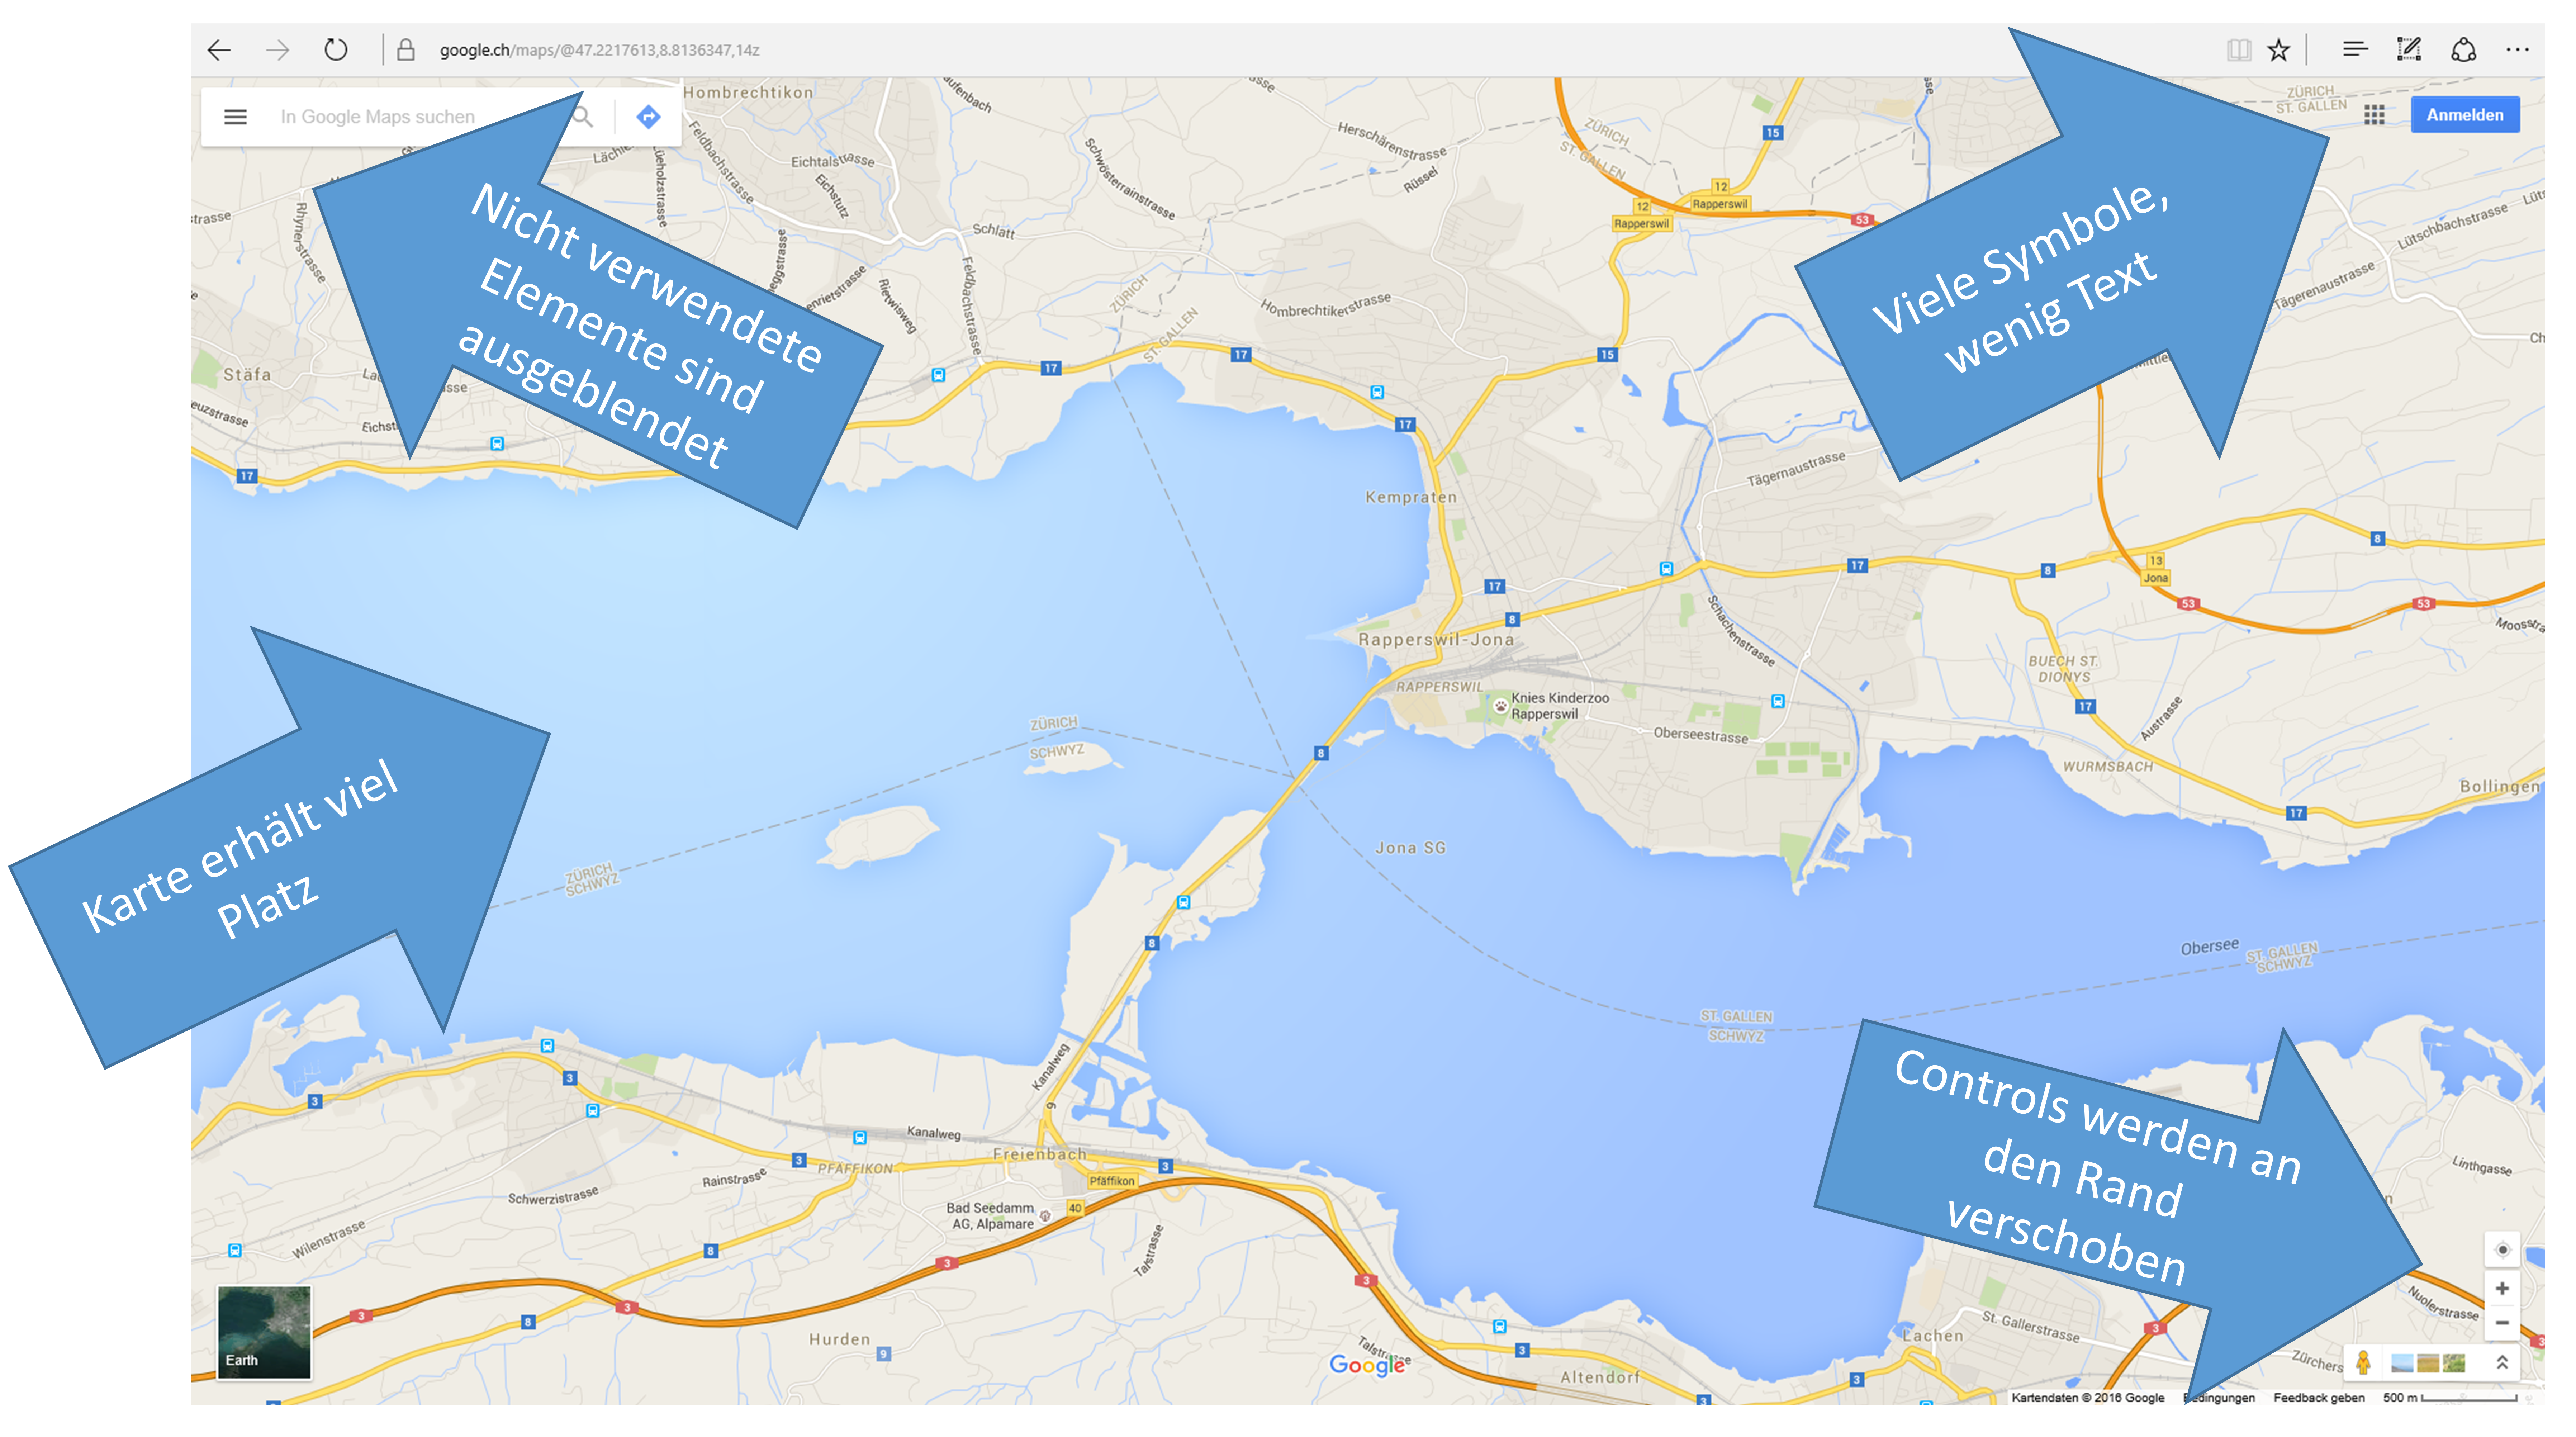
\includegraphics[height=7cm]{images/AnalyseGoogle.png}
\caption{Analyse Google Maps}
\label{fig:googlemaps}
\end{figure}
\noindent
Die Abbildung \ref{fig:googlemaps} zeigt die Auswertung der Analyse von Google Maps. Die Karte selbst, erhält sehr viel Platz und alle Bedienelemente (Controls) werden am Randbereich der Karte angeordnet. Dadurch ist sichergestellt, dass sich der Benutzer auf eine Kernaufgabe konzentriert und sich nicht ablenken lässt. Bei schlechteren Beispielen, auf denen die Karte nur wenig Platz erhält, fühlt sich der Benutzer sehr schnell eingegrenzt und muss deutlich mehr Aufwand ins Zoomen und seitlich Bewegen investieren. Dies kann einen Benutzer stören und ihn vom schnellen Erledigen der Aufgabe abhalten. Das User Interface passt sich laufend an die Nutzung des Benutzers an. Hat der Benutzer also einen Ort gefunden und möchten eine Route berechnen, wird ihm neu ein Menü eingeblendet, das ihm dies ermöglicht. Dadurch wird zwar der Karte Platz genommen, jedoch liegt nun das Hauptaugenmerk auf dem Planen der Route. Zusätzlich zum Einsparen von Platz werden bei den Bedienelementen meist kein Text sondern Symbole eingesetzt.
\subsubsection*{Ergebnisse Analyse}
Folgende Punkte, fliessen in das Design des Verkehrsmodell-Fallstudien-Editors mit ein:
\begin{itemize}
\itemsep0em
\item Der Karte viel Platz einräumen.
\item Menüs, welche nicht dem aktuellen Use Case entsprechen, ausblenden.
\item Viele Symbole, wenig Text.
\end{itemize}
\newpage
\subsubsection{ID Editor}
Der ID Editor von OpenStreetMap ist der bekannteste Editor für OpenStreetMap. Er bietet die Möglichkeit Daten von OpenStreetMap direkt auf einer Karte zu bearbeiten. Die Änderungen werden dann als Changeset an OpenStreetMap übertragen und freigeschaltet. Die Funktionalität des Verkehrsmodell-Fallstudien-Editors ähnelt sehr stark den Funktionen des ID Editors. Aufgrund dessen wurde das User Interface des ID Editors ebenfalls analysiert.
\begin{figure}[H]
\centering
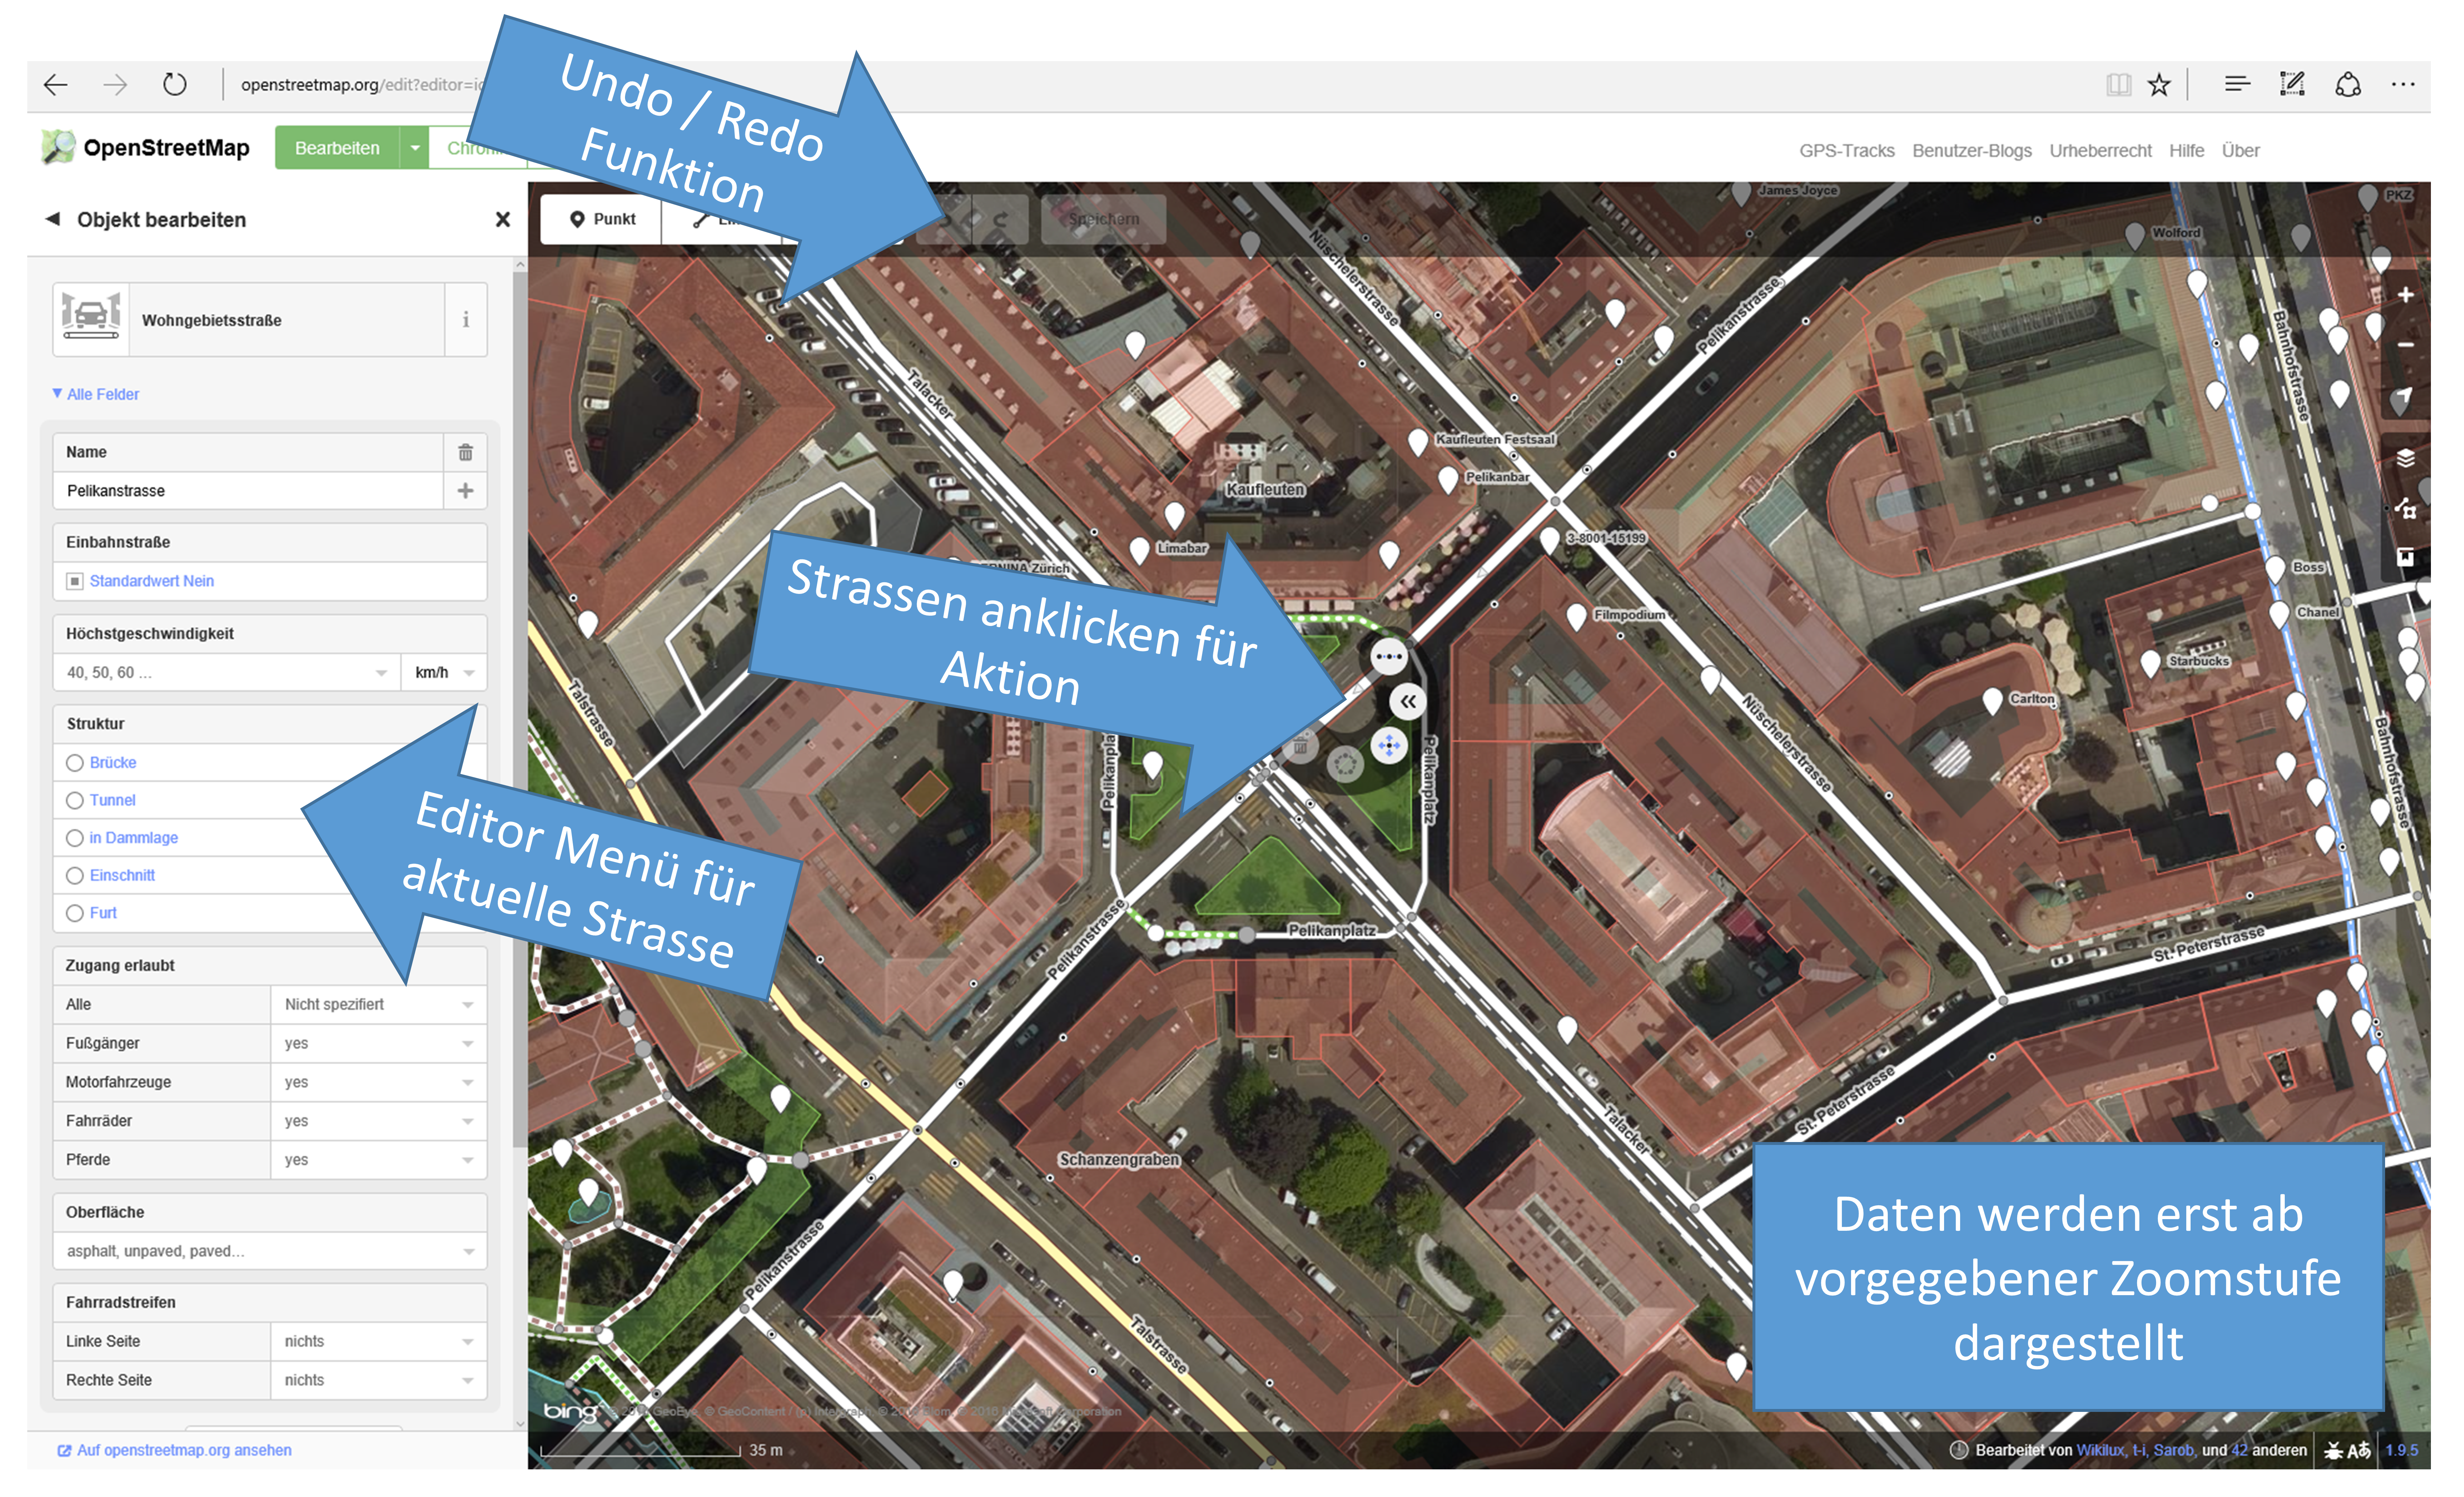
\includegraphics[height=7cm]{images/AnalyseIDEditor.png}
\caption{Analyse ID Editor}
\label{fig:ideditor}
\end{figure}
\noindent
Die Abbildung \ref{fig:ideditor} zeigt die Auswertung der Analyse des ID Editor. Eine Kerneigenschaft des User Interfaces ist es, dass die Daten erst ab einer gewissen Zoomstufe angezeigt werden. Dies hauptsächlich, weil der ID Editor eine deutlich grössere Datenmenge verarbeiten muss. Diese Eigenschaft ermöglicht es dem ID Editor, die Datenmenge, die zur selben Zeit dargestellt werden muss, auf ein Minimum zu reduzieren. Das Bearbeitungsmenü (Editor Menü) ist so aufgebaut, dass es nach dem Auswählen eines Elements die dazugehörigen Daten des Elements zur Bearbeitung anzeigt. Die Tatsache, dass die Karte dabei immer ersichtlich bleibt, ermöglicht eine leichte und schnelle Bedienung für den Benutzer. Eine weitere wichtige Funktion des ID Editors ist die Undo- / Redo-Funktion. Änderungen an Elementen können einfach wieder rückgängig gemacht werden oder dann wiederhergestellt werden.
\subsubsection*{Ergebnisse Analyse}
Folgende Punkte, fliessen in das Design des Verkehrsmodell-Fallstudien-Editors mit ein:
\begin{itemize}
\itemsep0em
\item Karte bleibt stehen, während Bearbeitung von Strassenattributen.
\item Bearbeitung der Strassen, durch Auswahl.
\item Undo- / Redo-Funktion.
\end{itemize}
\newpage
\subsubsection{Detail Konzept}\label{sec:detailuiconcept}
Aus den Erkenntnissen der Analyse von Google Maps und dem ID Editor wurde folgendes Konzept für das User Interface des Verkehrsmodell-Fallstudien-Editors entwickelt.
\begin{figure}[H]
\centering
\includegraphics[height=7cm]{images/KonzeptUI.png}
\caption{Wireframe Editor}
\label{fig:conceptui}
\end{figure}
\noindent
Angelehnt an Google Maps, wir das User Interface eine Karte besitzen, die den gesamten Platz im Browser ausfüllt. Die Bedienelemente, in der linken oberen Ecke, werden als selbsterklärende Symbole dargestellt und sind während der gesamten Benutzung der Applikation ersichtlich. Menüs, die zur Zeit nicht gebraucht werden, sind, wie in Abbildung \ref{fig:conceptui} dargestellt, ausgeblendet. Dies bietet dem Benutzer viel Platz, für das Suchen und Auswählen einer für ihn relevanten Strasse. Durch das Auswählen einer Strasse, wird ein Menü von der rechten Seite her eingeblendet, das das Bearbeiten der Parameter dieser Strasse ermöglicht (sh. Abbildung \ref{fig:concepteditStreet}).
\begin{figure}[H]
\centering
\includegraphics[height=7cm]{images/KonzeptEditStreet.png}
\caption{Wireframe Strassenattribute bearbeiten}
\label{fig:concepteditStreet}
\end{figure}
\newpage
\noindent
Um die Wegführung einer Strasse zu bearbeiten kann der Benutzer in einen Bearbeitungsmodus wechseln. In diesem Modus werden zusätzlich zu den Links auch die Nodes angezeigt, die ansonsten aus Performancegründen nicht geladen werden. Der Benutzer kann eine Strasse auswählen und dessen Führung mit Hilfe eines Menüs ändern.
\begin{figure}[H]
\centering
\includegraphics[height=7cm]{images/KonzeptChangeStreet.PNG}
\caption{Wireframe Strassenführung bearbeiten}
\label{fig:concepteditStreet}
\end{figure}
\noindent
Ein weiteres, naheliegendes Konzept für die Bearbeitung der Strassenführung, wäre ein Drag \& Drop Verfahren. Dieses Konzept wäre für den Benutzer am einfachsten, ist jedoch sehr zeitintensiv in der Implementation. Aus Zeitgründen musste dadurch auf Drag \& Drop verzichtet werden.
\section{Architektur}
\begin{figure}[H]
\centering
\includegraphics[height=12cm]{images/Architektur.png}
\caption{Tier des Verkehrsmodell-Fallstudien-Editor}
\label{tier_architecture}
\end{figure}
Aufgrund der Anforderungen bezüglich Performance und Antwortgeschwindigkeit an diese Arbeit, musste die Architektur für die Softwarelösung des Verkehrsmodell-Fallstudien-Editors skalierbar sein. D.h. es muss eine Entkopplung der Komponenten durchgeführt werden, die es erlaubt, die Last auf mehrere Server zu verteilen und dadurch eine höhere Last auf jedem einzelnen Server erlaubt.\\
Die Softwarelösung des Verkehrsmodell-Fallstudien-Editors ist als 3-Tier Applikation aufgebaut. Der Frontend-Tier ist eine Web Applikation, umgesetzt mit dem Play Framework. Der Backend-Tier wird als REST Service (Maturity Level 2 \cite{RESTMaturity}) mit Dropqizard entwickelt. Auf diesen Tier wird über einen Flux Load Balancer zugegriffen, der für die Skalierung verantwortlich ist. Dies erlaubt eine parallele Ausführung mehrerer Anfragen. Der letzte Tier, der Daten-Tier, wird durch eine PostgreSQL Datenbank bereitgestellt.
\begin{figure}[H]
\centering
\includegraphics[height=10cm]{images/layers.png}
\caption{Tier- / Layeraufteilung}
\label{fig:tierlayers}
\end{figure}
\noindent
Die Aufteilung der Presentation Logic auf den Client-Tier, sowie den Backend-Tier erlaubt es die Last der Datendarstellung auf die verschiedenen Komponenten zu verteilen. Die Vorbereitung und Aufbereitung der Daten wird vom Backend-Tier vorgenommen. Die Daten werden in einem, für den Client lesbaren, Format übertragen. Das Rendering der Daten übernimmt dann der Client.\\
In Abbildung \ref{fig:tierlayers} ist die gesamte Tier- und Layeraufteilung ersichtlich.
\section{SimMapEditor}
\begin{figure}[H]
\centering
\includegraphics[height=2cm]{images/presentationlayer.png}
\caption{SimMapEditor}
\label{fig:presentationlayer}
\end{figure}
\noindent
Der SimMapEditor ist die Frontend-Komponente der Architektur und basiert auf dem Play Framework. Der Client-Tier ist eine in Javascript entwickelte Software. Für die Abfrage der Daten, die auf der Karte dargestellt werden, greift sie auf den Backend-Tier zu. Das Rendering der Daten übernimmt ebenfalls der SimMapEditor. Er selbst besitzt keine eigene Business Logik, denn die ist komplett auf den Backend-Tier aufgelagert und dadurch nicht im Play Framework implementiert. Der SimMapEditor ist dafür zuständig, das User Interface Konzept (sh. \ref{sec:uiconcept} \nameref{sec:uiconcept}) sowie auch das Tiling der Daten (sh. \ref{ch:datentiles} \nameref{ch:datentiles}) zu implementieren und somit die Daten für die Karte vom Backend-Tier in Bereichen anfordert.
\section{SimMapService}
\begin{figure}[H]
\centering
\includegraphics[height=5.5cm]{images/BusinessLogicLayer.png}
\caption{SimMapService}
\label{fig:businesslogiclayer}
\end{figure}
\noindent
Der SimMapService stellt den Backend-Tier der Softwarelösung dar und ist in einer 3-Layer Architektur implementiert. Er wird als REST Service (Maturity Level 2 \cite{RESTMaturity}) entwickelt. Um dem Maturity Level 2 zu entsprechen, werden die Anfragen und Antworten des Services mit HTTP Standard Methoden und Codes ausgestattet. Mit den Codes wird dem Client angezeigt, welchen Status die Antwort besitzt. Z.B. wird bei einer erfolgreichen Anfrage, in der keine Daten in der Antwort enthalten sind, der HTTP Status Code \glqq{}204 - No Content\grqq{} zurückgesendet. Somit weiss der Client, dass die Anfrage erfolgreich war, jedoch keine Daten im Body enthalten sind. Für das Entgegennehmen, Verarbeiten und Aufbauen der Antworten mit den korrekten Codes ist die Presentation Logic Schicht des SimMapServices zuständig.\\
Die Application Logic Schicht des SimMapServices ist dafür zuständig, die Aufbereitungen, welche im Kapitel \ref{sec:concept_preprocessing} \nameref{sec:concept_preprocessing} beschrieben sind, durchzuführen. Zusätzlich lädt er Daten, je nach Zoomstufe und Koordinaten, aus der Resource Logic Schicht und bereitet diese auf. Anschliessend werden diese Daten an die Presentation Logic Schicht, für das Weiterleiten an den Client, weitergegeben.\\
Die Resource Logic Schicht bietet der Application Logic Schicht die Möglichkeit, auf die Daten in der Datenbank zuzugreifen. Die primäre Aufgabe dabei ist es, die Abfragen auf die Datenbank zu erstellen und durchzuführen.
\section{Datenbank}
Aufgrund der grossen Datenmenge, welche ein Verkehrsmodell umfassen kann, ist die Datenbank ein essenzieller Teil der Architektur. Das Datenmodell wurde darauf ausgelegt die Stammdaten, von den Daten der Changesets (sh. \ref{sec:changeset} \nameref{sec:changeset}) zu trennen.\\
\begin{figure}[H]
\centering
\includegraphics[height=10cm]{images/SimmapDatabase.jpg}
\caption{ERP der Datenbank}
\label{fig:databasescheme}
\end{figure}
\noindent
Die zentrale Komponente des Datenbankschemas, wie in Abbildung \ref{fig:databasescheme} ersichtlich, ist das Netzwerk. Das Netzwerk wird aus dem XML eingelesen, das über den Service importiert wurde. Jedes Netzwerk enthält sowohl Links als auch Nodes, die zusammen die Strassen des Verkehrsmodells bilden. In der Tabelle Network\textunderscore Options werden generelle Eigenschaften des Netzwerks, aus dem XML, gespeichert.\\
Die Tabellen Node\textunderscore Change und Link\textunderscore Change stellen ein Abbild der Tabellen Node und Link dar. In diese beiden Tabellen sowie auch der Tabelle Changeset werden die Daten eines Changesets abgespeichert. Dabei ist wichtig, dass lediglich die Differenz zu den originalen Datensätzen aus den Tabellen Link und Node abgespeichert werden. Die restlichen Spalten werden auf null gesetzt.\\
Das Datenmodell enthält bewusst einige Redundanzen. Die Koordinaten der Nodes werden aus Performancegründen sowohl direkt auf dem Node als auch in den dazugehörigen Links abgespeichert. Im Kapitel \ref{ch:redundance} \nameref{ch:redundance} werden die Gründe dazu, genauer erläutert.
\chapter{Implementation}
Für die Implementation dieser Bachelorarbeit wurden die im vorherigen Kapitel \ref{ch:konzepte_architektur} \nameref{ch:konzepte_architektur} beschrieben Konzepte angewendet.
\section{XML Daten Import}
Um mit den grossen Datenmengen in den vorhandenen XML Dateien effizient zu arbeiten, müssen diese Daten in eine Datenbank importiert werden. Dafür wurde ein Import Formular im Web Interface integriert, das im Hintergrund die Daten an einen Web Service sendet, der für den Import zuständig ist. Die Daten werden direkt beim Import aufbereitet, sodass die Abfrage der Daten schneller ist.
\section{Tiling der Daten}
\label{sec:tilingdataimplementation}
Während des Imports werden zwei verschiedene Vorberechnungen durchgeführt. Mit Hilfe dieser Aufbereitung ist es möglich, die Daten effizienter zu filtern. Dadurch wird die Antwortzeit einer Anfrage deutlich verkürzt.
\subsection{QuadKey}
Die erste Vorbereitung ist die Berechnung des QuadKeys. Wie in Kapitel \ref{ch:datentiles} \nameref{ch:datentiles} beschrieben, können mit Hilfe des QuadKey einzelne Bereiche der Welt eindeutig identifiziert werden. Wenn nun eine Anfrage an den Server gesendet wird, in der die Daten eines spezifischen QuadTiles angefordert werden, müssen die Links ebenfalls einen QuadKey besitzen, um danach zu filtern. Dafür werden die QuadKeys der beiden Nodes berechnet, die zu einem Link gehören. Der gemeinsame Präfix stellt nun den kleinstmöglichen QuadKey dar, in den der gesamte Link hineinpasst.\\
Wie in Abbildung \ref{pic:example_quadtile} bei Link 2 ersichtlich, kann eine Strasse in einem QuadTile ersichtlich sein, ohne dass sich beide Nodes in diesem Quadtile befinden. In diesem Beispiel hat Link 1 einen QuadKey von 010 und Link 2 von 01. Damit nun der Link 2 bei einer Abfrage der Daten des QuadTiles 010 auch mitgeliefert wird, müssen alle Strassen, die einen QuadKey besitzen, der einen Prefix des angeforderten QuadKeys darstellt, auch mitgeliefert werden. D.h. dass nun für die Abfrage des QuadTiles 010 alle Strassen, die den QuadKey 010, 01, 0 oder sogar einen leeren QuadKey (\glqq{}\grqq{}) besitzen mitgeliefert werden.
\begin{figure}[H]
\centering
\includegraphics[height=9cm]{images/QuadTile_example.PNG}
\caption{Beispiel QuadTile}
QuadKey Link 1: 010\\QuadKey Link 2: 01
\label{pic:example_quadtile}
\end{figure}
\noindent
Der QuadKey ist eine sehr gute Technik um die Daten auf der Karte zu adressieren und dadurch eine Filterung der Daten durchzuführen. Zudem stellt diese Technik sicher, dass alle in einem gewissen QuadTile ersichtlichen Links sicher mitgeliefert werden.\\
Ein Nachteil dieser Technik ist es, dass bei höheren Zoomlevels Daten mitgeliefert werden, die bei einem vorherigen QuadTile bereits mitgeliefert wurden. Das User Interface verhindert zwar das neue Zeichnen von Duplikaten, jedoch werden dadurch Datensätze übertragen, die bereits gezeichnet sind und dadurch überflüssig sind. In den für diese Arbeit zur Verfügung stehenden Modellen hält sich die Menge von Links, die einen kleinen Präfix besitzen in Grenzen. Dadurch ebenfalls die Menge an Links, die mehrfach übertragen werden oder ausserhalb des sichtbaren Bereichs gezeichnet werden.
\newpage
\subsection{MinLevel}
Zusätzlich zu dem QuadKey wird beim Import für jeden Link der Mindest-Level (MinLevel) berechnet. Denn nur mit dem QuadKey würden alle Strassen in der aktuell angezeigten Bounding Box geladen werden, auch die eher kleineren Nebenstrassen. Aus diesem Grund wird beim Import ein MinLevel berechnet, der besagt, ab welchem Zoom Level in der Karte diese Strasse geladen wird. Dadurch ist es möglich, eine Strasse nach ihrer Wichtigkeit zu beurteilen und erst ab einem bestimmten Zoomlevel anzuzeigen.\\
Bei der Berechnung dieses Mindest-Levels wird in erster Linie auf die maximale  Geschwindigkeit geachtet. Die Geschwindigkeit sagt sehr viel über die Wichtigkeit der Strasse selbst aus. Eine Strasse mit einer hohen maximalen Geschwindigkeit, wie z.B. eine Autobahn, wird in diesem System als wichtig erachtet und dadurch bereits auf einem niedrigeren Zoomlevel angezeigt. Beim Level 10 und 14 wurden noch weitere Kriterien verwendet, um eine feinere Skalierung zu erhalten.\\
Der MinLevel einer Strasse wird wie folgt berechnet:\\[0.3cm]
\begin{tabular}{l c l} 
Level 10 & => & Geschwindigkeit > 30 m/s und Anzahl Spuren > 2 \\ 
Level 11 & => & Geschwindigkeit > 30 m/s  \\ 
Level 12 & => & Geschwindigkeit > 23 m/s \\ 
Level 13 & => & Geschwindigkeit > 14 m/s \\ 
Level 14 & => & Geschwindigkeit > 13 m/s und Kapazität >= 4000  \\ 
Level 15 & => & Geschwindigkeit > 13 m/s \\ 
Level 16 & => & Der Rest \\ 
\end{tabular}\\[0.4cm]
Alternativ zu den verwendeten Kriterien könnte die Berechnung des MinLevels auch mit Hilfe der Kapazität und zur feineren Abstufung der Anzahl Spuren der einzelnen Strassen durchgeführt werden. Dieses Verfahren hat jedoch eine unregelmässigere Verteilung auf die einzelnen Zoomlevels zur Folge. Aus diesem Grund wurde das Verfahren mit der Geschwindigkeit gewählt.
\newpage
\section{User Interface - Implementation}
Wie in Kapitel \ref{sec:uiconcept} \nameref{sec:uiconcept} beschrieben, muss das User Interface des Verkehrsmodell-Fallstudien-Editors einigen Anforderungen entsprechen. Dieses User Interface wird als Javascript Single Page Anwendung konzipiert und implementiert. Dies hat zum Vorteil, dass der Benutzer die Seite nie wechselt, sondern alle benötigten Elemente laufend nachgeladen werden. Dadurch erhält der Benutzer eine flüssigere User Experience. Die Web Applikation wird in eine Main View (Haupt-Anzeige) und mehrere Partial Views (Teil-Anzeigen) aufgeteilt. Die Partial Views werden im Play Framework als Route erfasst und mittels Javascript angefordert. Anschliessend werden diese Partial Views in einen Container geladen. Die Abbildung \ref{fig:mainviewpartialview} zeigt den Aufbau des User Interface mit einer eingezeichneten Partial View.
\begin{figure}[H]
\centering
\includegraphics[height=6cm]{images/Mainviewpartialview.png}
\caption{User Interface mit eingezeichneter Partial View}
\label{fig:mainviewpartialview}
\end{figure}
\noindent
Wie in Abbildung \ref{fig:mainviewpartialview} ersichtlich, wurde der Karte viel Platz eingeräumt. Für die Darstellung der Karte wurde das Framework Leaflet \cite{Leaflet} sowie d3.js \cite{D3JS} verwendet. In der Kombination erlauben diese Frameworks die Erstellung einer Karte mit beliebigem Kartenmaterial im Hintergrund. Für die Karte wurde ein eigenes Kartendesign über Mapbox\cite{Mapbox} erstellt. Um zusätzlich zu der Karte eine Schicht mit den Daten aus dem Verkehrsmodell darzustellen, musste eine Erweiterung für Leaflet (TileLayer GeoJSON \cite{LeafletGeoJSON}) verwendet werden. Diese Erweiterung ermöglicht es, eine Schicht aufzubauen, welche die Daten für die Darstellung von einer URL nach dem OpenStreetMap Schema (x, y , zoom) anfordert und dabei GeoJSON als Antwortformat erwartet. Diese Library wurde gemäss den Anforderungen des Verkehrsmodell-Fallstudien-Editors erweitert. Mit Hilfe dieser Libray konnte das Konzept des Tiling der Daten (vgl. \ref{ch:datentiles} \nameref{ch:datentiles}) umgesetzt werden. Für die Interaktionen mit den einzelnen Editoren wird AngularJS \cite{AngularJS} Version 1.5 verwendet. AngularJS ermöglicht das Binding eines Models an Datenfelder und dadurch auch das Bearbeiten dieser Models. Z.B. wird beim Anklicken einer Strasse das Model der Strasse an das Edit-Menü gebunden und ermöglicht dadurch die Bearbeitung (vgl. Abbildung \ref{fig:editstreetattributes}).
\begin{figure}[H]
\centering
\includegraphics[height=6cm]{images/EditStreetattributes.png}
\caption{User Interface mit geöffnetem Editor für Strassenattribute}
\label{fig:editstreetattributes}
\end{figure}
\noindent
Um die Wegführung einer Strasse zu bearbeiten, kann eine Strasse angeklickt werden. Dabei öffnet sich ein Bearbeitungsfenster, in dem der Start und Endpunkt der Strasse mittels Klick auf den entsprechenden Node bearbeitet werden kann (vgl. Abbildung \ref{fig:editstreetdirection}). Nach der Bearbeitung wird die Strasse neu gezeichnet und hervorgehoben.\\
\begin{figure}[H]
\centering
\includegraphics[height=6cm]{images/EditStreetdirection.png}
\caption{User Interface mit geöffnetem Editor für Strassenführung}
\label{fig:editstreetdirection}
\end{figure}
\noindent
Änderungen, welche über den Attribut-  oder Strassenführungseditor erstellt werden, werden auf einem Undo-Stack abgelegt. Dadurch können Änderungen über eine Undo-Funktion wieder rückgängig gemacht werden und über ein Redo wiederhergestellt werden. Das Changeset sowie der Undo- und Redo-Stack sind im Session Storage des Browser abgelegt. Dadurch gehen die Änderungen nicht verloren, solange die Browser Session noch offen ist. Wird der Browser geschlossen, gehen die Änderungen durch die Löschung der Session verloren. Der Benutzer kann seine Änderungen speichern, so dass sie in der Datenbank persistiert werden. Der Vorteil des Session Storage liegt darin, dass ein Benutzer die Seite neu laden kann oder ein Tab schliessen kann, ohne dass seine lokalen Änderungen verloren gehen.
\section{Performance Optimierungen}
\label{ch:performance}
Die Performance ist ein sehr wichtiger Faktor in dieser Arbeit. Ohne starke Performance kann die grosse Datenmenge in diesem Projekt nicht effizient dargestellt werden. Aufgrund dessen wurde einiges an Zeit in die Optimierung investiert. Zwei wichtige Faktoren haben grossen Einfluss auf die Performance dieser Web Applikation. Zum einen ist dies die Antwortzeit der einzelnen Abfragen der Daten. Diese Antwortzeit konnte durch mehrere Optimierungen, die in diesem Kapitel genauer beschrieben werden, deutlich verbessert werden. Dadurch konnten die nicht-funktionalen Anforderungen aus dem Kapitel \ref{ch:NFRs} \nameref{ch:NFRs} eingehalten werden.\\
Ein weiterer grosser Faktor ist das Rendering der Daten im Browser. In höheren Zoomlevels werden bis zu mehreren Tausend Links und Nodes im Browser dargestellt. Der Browser benötigt für das Rendering dennoch eine gewisse Zeit, auf die der Entwickler keinen grossen Einfluss hat. Es kann lediglich darauf geachtet werden, dass keine redundante Informationen vom Browser gerendert werden müssen.
\subsection{Caching}
Für die Anzeige der Strassen und Nodes werden sehr viele Daten übertragen. Damit die Daten bei mehrmaligem Anfragen nicht jedes Mal übertragen werden müssen, wird clientseitiges Caching eingesetzt.\\
Der Server gibt dem Client vor, wie er die Daten zwischenspeichern soll. Dafür wird bei jeder Antwort ein maximales Alter der Daten gesetzt. Wie in Abbildung \ref{pic:browser_cache} ersichtlich, speichert der Client die Daten in seinen lokalen Zwischenspeicher (Cache) und verwendet diese, solange das maximale Alter von einer Stunde noch nicht erreicht ist. Dies macht Sinn, weil sich die Stammdaten des Verkehrsmodells nur sehr selten ändern. Erst nach Ablauf dieser Stunde sendet der Browser erneut eine Anfrage an der Server.
\begin{figure}[H]
\centering
\includegraphics[height=6cm]{images/browser_cache.jpg}
\caption{Browser Zwischenspeicher Request (Cache) \cite{HTTPCacheHeaders}}
\label{pic:browser_cache}
\end{figure}
\newpage
\noindent
Nun liegt es am Server zu prüfen, ob die Daten, die sich im Cache des Clients befinden, noch aktuell sind. Dafür wird mit einem HTTP Entity Tag gearbeitet \cite{WikipediaETag}. Dieser setzt sich aus der x- und y-Koordinate, dem Zoom Level sowie aus dem Zeitstempel der letzten Bearbeitung der Daten zusammen. Durch diese unterschiedlichen Informationen ist der Entity Tag für jeden QuadTile eindeutig. Durch das zusätzliche Verwenden des Zeitstempels ist auch sichergestellt, dass sich der Entity Tag unterscheidet, sobald eine Änderung in den angeforderten Stammdaten auf dem Server vorliegt.\\
Jede Antwort, die zuvor an den Client gesendet wurde, wird mit diesem HTTP Entity Tag versehen. Beim erneuten Anfragen der Daten, wird dieser Entity Tag vom Client mitgesendet und mit dem berechneten, aktuellen Entity Tag der Daten auf dem Server verglichen. Wie in Abbildung \ref{pic:browser_etag} ersichtlich, wird vom Server der HTTP Status 304 (Not Modified) \cite{W3HttpStatus} gesendet, falls diese identisch sind. Dadurch weiss der Client, dass seine Daten noch aktuell sind. Wurden die Stammdaten auf dem Server geändert, stimmen die Entity Tags aufgrund des Zeitstempels der letzten Bearbeitung nicht mehr überein und der Server sendet die neuen Daten an den Client. Diese Daten werden dann vom Client wieder für eine Stunde zwischengespeichert und anschliessend beginnt der Prozess von vorne. Dieses Caching kann zu einer Inkonsistenz der Daten im Cache und dem Server führen. Jedoch wurde dieses Risiko bewusst eingegangen weil ein Update der Stammdaten nur sehr selten vorkommt. Zudem kann ein Update der Stammdaten zeitlich so gelegt werden, dass die Benutzer davon nicht betroffen sind.
\begin{figure}[H]
\centering
\includegraphics[height=6cm]{images/browser_etag.jpg}
\caption{HTTP Entity Tag Request \cite{HTTPCacheHeaders}}
\label{pic:browser_etag}
\end{figure}
\noindent
Durch dieses Verfahren ist sichergestellt, dass das Übertragen von Daten möglichst reduziert wird und dadurch Performance gewonnen wird. Das Beantworten eines Requests, der noch den selben Entity Tag verwendet und somit im Cache noch aktuell ist, benötigt ca. 50ms. Hingegen das erneute Senden würde ca. 200ms bis 300ms benötigen. Dadurch ist das Beantworten um de Faktor vier bis sechs schneller. Diese gewonnene Performance wird erst beim längeren Verwenden der Applikation ersichtlich, sobald bereits geladene Daten nicht mehr erneut geladen werden müssen.
\newpage
\subsection{Erneutes Zeichnen}
Die verwendete Library \glqq{}Leaflet GeoJSON Tile Layer\grqq{} \cite{LeafletGeoJSON}, die für das Abfragen der Daten in Tiles verantwortlich ist, wurde standardmässig so entwickelt, dass die Daten auf jedem Zoom Level neu gezeichnet werden. Im Rahmen dieser Arbeit wurde die Funktionalität erweitert, so dass die Strassen beim Hineinzoomen bestehen bleiben und lediglich die neuen Strassen dazu gezeichnet werden. Ebenfalls wurde die Library so angepasst, dass  beim Herauszoomen alle Strassen, die auf einem höheren Zoomlevel gezeichnet wurden, wieder entfernt werden. Dafür werden alle Schlüssel der gezeichneten Strassen mit dem dazugehörigen Zoomlevel, auf dem sie gezeichnet wurden, in eine Map< Zoomlevel, List<Schlüssel> > abgelegt. Dadurch kann die Library beim Herauszoomen alle Schlüssel, die zu einem Zoomlevel gehören, löschen.
\subsection{Datenbank Index}
Der Verkehrsmodell-Fallstudien-Editor arbeitet mit einer grossen Datenmenge, die in einer Datenbank gehalten wird. Die Abfrage einer Teilmenge der Daten benötigte bei einer Datenmenge von 4 Millionen Datensätzen bis zu drei Sekunden. Diese Antwortzeit ist deutlich zu lange und eine Auswertung des Ausführungsplans zeigte, dass die Indizes, die auf die einzelnen Zeilen gesetzt sind, nicht verwendet wurden.\\
Die Abfrage der Strassen beinhaltet eine LIKE Abfrage von SQL, die das Suchen von Strassen mit QuadKeys ermöglicht, die den QuadKey des aktuellen Tiles als Prefix besitzen. Speziell für SQL Abfragen mit einem LIKE Operator, bietet PostgreSQL eine Operator Klasse \glqq{}varchar\textunderscore pattern\textunderscore ops\grqq{}, die zusätzlich auf den Index des QuadKeys gesetzt werden kann. Dadurch wird der Index speziell für solche LIKE Abfragen vorbereitet und deutlich schneller. Nach dem Hinzufügen dieser Operator Klasse war der Zugriff auf die Daten zehn Mal so schnell und wir erreichten eine Zugriffszeit zwischen 100ms und 300ms.
\subsection{Datenbank Redundanz} \label{ch:redundance}
Die Daten in der Datenbank sind in eine Tabelle \glqq{}Links\grqq{} und eine Tabelle \glqq{}Nodes\grqq{} aufgeteilt. Bei der Abfrage werden sowohl die Parameter des Links als auch die Koordinaten der dazugehörigen Nodes benötigt. Dafür wurde zu Beginn ein klassischer SQL JOIN verwendet, um die beiden Tabellen miteinander zu verknüpfen. Durch die Analyse des Ausführungsplans wurde ersichtlich, dass dieser JOIN ca. die Hälfte der Ausführungszeit in Anspruch nahm. Um diese Zeit einzusparen, werden nun die Koordinaten der beiden Nodes direkt beim Import der Daten in die Tabelle der Links mit abgespeichert. Dadurch sind die Koordinaten der Nodes zwar redundant vorhanden, jedoch beschleunigt dies die Abfrage um den Faktor 2. Daher wurde die Redundanz der Daten in Kauf genommen.
\newpage
\section{Infrastruktur}
evtl. TODO
\subsection{Docker}
evtl. TODO
\subsection{Load Balancing}
evtl. TODO
\chapter{Resultate}
\section{Performance}
Wie in Kapitel \ref{ch:NFRs} \nameref{ch:NFRs} beschrieben, ist die Performance eine der wichtigsten nicht-funktionalen Anforderungen. Dies hatte zur Folge, dass besonders viel Zeit in dessen Optimierung investiert wurde. In Kapitel \ref{ch:performance} \nameref{ch:performance} wird genauer auf die durchgeführten Optimierungen eingegangen.\\
Grundsätzlich gab es drei verschiedene Stufen von Performance, die erreicht wurden. In diesem Kapitel werden diese vier Stufen genauer analysiert und beschrieben.
\subsubsection*{Stufe 1}
In der ersten Stufe, zu Beginn des Projektes, wurde das gesamte Verkehrsmodell-Netzwerk mittels einer einzigen Abfrage beim Öffnen der Applikation geladen. Dabei wurde mit dem öffentlichen Netzwerk von Santiago de Chile gearbeitet. Dies beinhaltet ca. 60'000 Datensätze. Gemäss Tests benötigte diese Abfrage im Durchschnitt ca. 6 Sekunden. Mittels dieser Vorgehensweise wäre es unmöglich gewesen, ein Netzwerk wie die Schweiz, mit ca. 4 Millionen Datensätzen, auf dieser Applikation zu laden und anzuzeigen.
\subsubsection*{Stufe 2}
In der nächsten Stufe 
\subsubsection*{Stufe 3}
\subsubsection*{Stufe 4}
v0.2:
Arbeitete noch mit Santiago, Lädt das komplette JSON mit ca. 60'000 Datensätzen
Benötigt für das Laden dieser Datensätze:
5954 ms
5717 ms
5951 ms
5978 ms
6175 ms
6184 ms
6204 ms
5924 ms
6058 ms
5882 ms
-------
60'027 ms / 10 = 6002,7 ms

Browser würde mit 4 Millionen Datensätzen komplett crashen.

v0.3:
Vorher:
Bei tiefen Zoomlevel:
1000ms - 3000ms
Bei höheren Zoomlevel:
3000ms - 10000ms

Nach dem entfernen von JOINS und Hinzufügen von Index
Bei tiefen Zoomlevel:
50ms - 100ms
Bei höheren Zoomlevel:
50ms - 300ms

v0.4:
Performance deutlich höher:
bei tiefen Zoomlevel:
50ms - 100ms
bie höheren Zoomlevel:
50ms - 300ms

\section{Rückblick Technologien}
\subsection*{Leaflet}
\subsection*{Leaflet GeoJSON Tile Layer}
\subsection*{AngularJS}
\subsection*{Play Framework}
\subsection*{Dropwizard}

\chapter{Schlussfolgerung}
\section{Erkenntnisse}
\begin{flushleft}
TODO
\end{flushleft}
\section{Weiterführung der Arbeit}
\begin{flushleft}
TODO
\end{flushleft}
\section{Persönliches Fazit}
\subsection{Dominik Heeb}
\begin{flushleft}
TODO
\end{flushleft}
\subsection{Fabian Keller}
\begin{flushleft}
TODO
\end{flushleft}
( Future works)
% List of figures & glossary
%%%%%%%%%%%%%%%%%%%%%%%%%%%%
\listoffigures
\glsaddall
\printglossary[style=altlist,title=Glossar]

% Bibliography
%%%%%%%%%%%%%%
\bibliographystyle{alpha}
\nocite{*}
\bibliography{index/bibliography}


% Attached sources
%%%%%%%%%%%%%%%%%%
% \input{attachments/attachments}


\end{document}